\section{Speed Reference Output Channel}

	\subsection{Speed Control}
		\par
		For the braketests, somethings as important as measuring the speed of the rotor is controlling it, as mentioned in Subsection \ref{ssec:lowerLayerlHardware}. The rotor speed can be controlled in two ways:
			\begin{itemize}
				\item First way is the deceleration of the rotor with the aid of the brake system using the brake pads.
				\item Second way of controlling it by accelerating the rotor with the aid of the electric engine.
			\end{itemize}
		The electric engine used is a alternate current three-phase type, it in order to control it's speed a frequency inverter was used. The frequency inverter has many different controlling interfaces that lead to manipulating the three-phase electric system in order to control the engine's rotationary speed.
		\par
		In this project the frequency inverter used was the \textit{Weg CFW-08} \cite{wegCFW08Manual}, one way of controlling the speed of the rotor using this device is by using it's analog input, it can be configured as a notch to ten volts input that has a linear proportion to the the output frequency that goes to the engine, that way the problem to figure out in this solution is how to implement a analog output from a microcontroller that only has digital outputs.

		\begin{figure}[htbp]
			\centering
				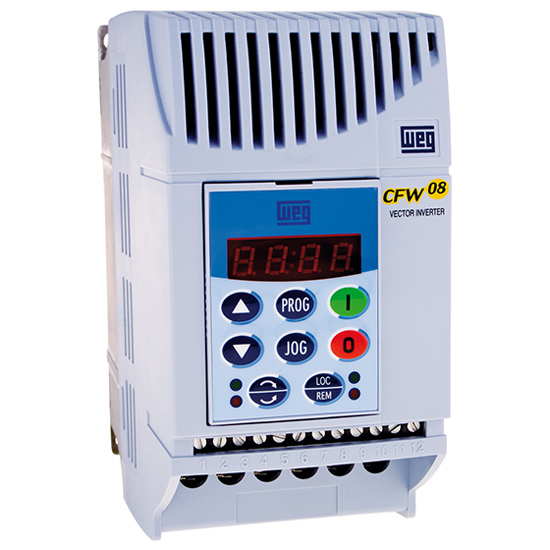
\includegraphics[scale=0.4]{figuras/fig-wegCFW08}
			\caption{Weg CFW-08 Frequency Inverter \cite{fig-wegCFW08}}
			\label{fig:wegCFW08}
		\end{figure}

	\subsection{Filter characteristics definition}\label{ssec:filterCharacteristicsDefinition}
		\par
		Fortunately the microcontroller has pre-configured PWM \textit{(Pulse Width Modulation)}, as explained in Subsection \ref{ssec:pwm}, a PWM signal can encode a analog voltage value proportional to it`s duty cycle, and this is usually done with the aid of a low pass filter that will extract this analog voltage from the PWM signal. As said in the previous paragraph the frequency inverter used in this project is the \textit{Weg CFW-08}, and it's analog input has a zero to ten voltage input with eight bits of resolution. We can calculate the minimal voltage difference that will change the output frequency of the device using Voltage, in which $\Delta V$ is the minimal voltage difference, $V_{max}$ is the maximum voltage and \textit{"n"} is the number of bits of the input resolution.

			\begin{equation}\label{eqn:minVoltage}
				\Delta V=\frac{V_{max}}{2^{n}}
			\end{equation}
	
		As mentioned in Section \ref{sec:mcu-hw}, the choosen MCU has a five volts high logic level, this voltage level will need amplification in order to best suit the zero to ten volts input from the frequency inverter. According to \cite{alter2008pwm}, converting a PWM signal to a analog voltage generates a constant voltage ripple. It was decided to amplify this voltage prior to filtering because this way the voltage ripple generated from the filtering stage will not be amplified. Using a OPAMP and two resistors it is possible to convert a five volts amplitude square wave (PWM wave) to a 10V amplitude wave by giving a gain of two to the input signal. Using Equation \ref{eqn-gain-neg-closed-loop-amp} from Sub-section \ref{ssec:closed-loop-amplifier}, it is possible to achieve the desired gain of two using both R$_{f}$ and R$_{g}$ of 10k$\Omega$ as Figure \ref{fig:closed-loop-opamp} shows how to.

		The maximum ripple is the $\Delta V$ from Equation \ref{eqn:minVoltage}. Equation \ref{eqn:atte} \cite{metivier2013pwm} gives the necessary $\frac{dB}{decade}$ attenuation to guarantee a PWM converted signal desired ripple.

	 		\begin{equation}\label{eqn:atte}
				A_{dB}=20\cdot log \left( \frac{V_{RIPPLE}}{V_PWM} \right) 
			\end{equation}
			
		As the $V_{PWM}$ will already be aplified prior to filtering, $V_{PWM}=V_{max}$, this will produce the following Equation \ref{eqn:attenuation}.
		
			\begin{equation}\label{eqn:attenuation}
				A_{dB}=-20 \cdot n \cdot log \left( 2 \right) 
			\end{equation}
	
		And Equation \ref{eqn:LPFcuttoffFrequency} \cite{metivier2013pwm}, is used to calculate the maximum needed cuttoff frequency for the further to be designed LPF (\textit{Low-Pass-Filter}) in order to convert the PWM signal to a analog voltage. This cutoff frequency can not be to much smaller than the one calculated otherwise this will have negative consequences to the output signal \cite{keim2016pwm}. The slope value is the filter slope and for first order filters and second order filters this slope value is equal respectively to 20dB/decade and 40dB/decade \cite{metivier2013pwm}.
	
			\begin{equation}\label{eqn:LPFcuttoffFrequency}
				f_{c}=f_{PWM} \cdot 10^{-\frac{A_{dB}}{Slope}}
			\end{equation}

		It is possible to combine all this equations into one single equation to calculate the needed cutoff frequency, is this done in Equation \ref{eqn:LPFcuttoffFrequency2}.

			\begin{equation}\label{eqn:LPFcuttoffFrequency2}
				\begin{split}
					f_{c}=f_{PWM} \cdot 10^{-\frac{A_{dB}}{Slope}}	\\
					f_{c}=f_{PWM} \cdot 10^{-\frac{-20 \cdot n \cdot log \left( 2 \right)}{Slope}}	\\
					f_{c}=f_{PWM} \cdot 10^{log \left( 2^{\frac{20 \cdot n }{Slope}} \right)}	\\
					Knowing:	\\
					x \cdot log \left( A \right) =  log \left( A^{X} \right) \\
					10^{log \left( A \right) } = A	\\
					So:	\\
					f_{c}=f_{PWM} \cdot  2^{\frac{20 \cdot n}{Slope}}
				\end{split}
			\end{equation}

	
		As shown in Appendix \ref{app:microCode}, the PWM frequency was defined so $f_{PWM}=62.5kHz$, also $n=8$ and as according to \cite{metivier2013pwm}, a second order LPF is better for converting a PWM signal to voltage and it has by default $Slope=-40dB/decade$, using Equation \ref{eqn:LPFcuttoffFrequency2} it is possible to calculate a maximum cutoff frequency of 3906.25Hz. 

	\subsection{Sallen-Key Low Pass Active Filter}
	
		The Sallen-Key LPF setup is probably one of the best second order filters architectures available \cite{dorfSvodoba2014}, this setup is displayed on Figure \ref{fig:sallenKeyLPF}.

		\begin{figure}[htbp]
			\centering
				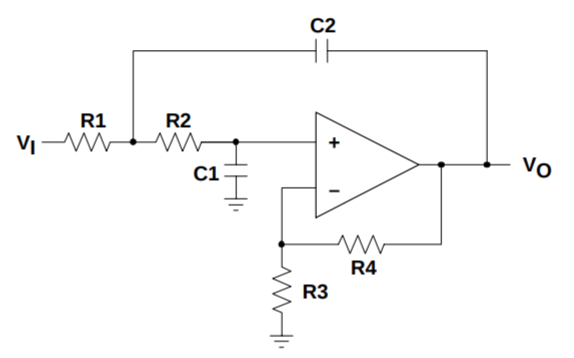
\includegraphics[scale=0.6]{figuras/fig-sallenKeyLPF}
			\caption{Sallen-Key Active Low Pass Filter \cite{texas1999sallenkey}}
			\label{fig:sallenKeyLPF}
		\end{figure}

				According to \cite{texas1999sallenkey}, this filter setup has a cutoff frequency defined by Equation \ref{eqn:sallenKeyTransferFunction}, quality factor (Q) defined by Equation \ref{eqn:sallenKeyQ}, gain (k) defined by Equation \ref{eqn:sallenKeyK} and cutoff frequency giver by Equation \ref{eqn:sallenKeyCutoffFrequency}.

		\begin{equation}\label{eqn:sallenKeyTransferFunction}
			H(s)=\frac{k}{s^{2} \cdot \left( R_{1} \cdot R_{2} \cdot C_{1} \cdot C_{2} \right) + s \cdot \left( R_{1} \cdot C_{1} + R_{2} \cdot C_{1} + R_{1} \cdot C_{2} \cdot \left( 1 - k \right) \right) + 1} 
		\end{equation}

		\begin{equation}\label{eqn:sallenKeyQ}
			Q=\frac{\sqrt{R_{1} \cdot R_{2} \cdot C_{1} \cdot C_{2}}}{R_{1} \cdot C_{1} + R_{2} \cdot C_{1} + R_{1} \cdot C_{2} \cdot \left( 1 - k \right)}
		\end{equation}

		\begin{equation}\label{eqn:sallenKeyK}
			k = 1 + \frac{R_{3}}{R_{4}}
		\end{equation}

		\begin{equation}\label{eqn:sallenKeyCutoffFrequency}
			f_{c}=\frac{1}{2 \cdot \pi \sqrt{R_{1} \cdot R_{2} \cdot C_{1} \cdot C_{2}}} 
		\end{equation}


		A useful design strategy is to set $R_{1}= m \cdot R$, $R_{2}=R$, $C_{1}=C$ and $C_{2}= n \cdot C$. Replacing this values in Equation \ref{eqn:sallenKeyQ} gives a new Equation \ref{eqn:sallenKeyQ2}.

		\begin{equation}\label{eqn:sallenKeyQ2}
			Q=\frac{\sqrt{m \cdot n}}{m + 1 - m \cdot n}
		\end{equation}

		The quality factor of a Sallen-Key filter is influenced by the gain (k) and defines the dB gain on the cutoff frequency, ideally this factor should be closer as possible to $\frac{\sqrt{2}}{2}$ \ref{dorfSvodoba2014}. Setting a arbitrary value of $m=2$, the ideal value of $Q=\frac{\sqrt{2}}{2}$ and using Equation \ref{eqn:sallenKeyQ2} it is possible to calculate a $n=0,6771$. It is possible to simplify Equation \ref{eqn:sallenKeyCutoffFrequency} using the same method used to simplify Equation \ref{eqn:sallenKeyQ} to \ref{eqn:sallenKeyQ2}. Using this method will produce Equation \ref{eqn:sallenKeyRC} that will be used to determine the $R \cdot C$ constant that will be later used to define the resistors and capacitor values of our filter. 

		\begin{equation}\label{eqn:sallenKeyRC}
			R \cdot C = \frac{1}{2 \cdot \pi f_{c} \cdot \sqrt{m \cdot n}}
		\end{equation}

		Using the previously calculated values for \textit{m}, \textit{n}, \textit{$f_{c}$} and Equation \ref{eqn:sallenKeyRC} wil give us a $R \cdot C = 3.50115 \cdot 10^{-5}$. Setting a arbitrary value of $R=10 \cdot 10^{3}$ will lead to $C=3.5 \cdot 10^{-9}$. Using the relations: $R_{1}= m \cdot R$, $R_{2}=R$, $C_{1}=C$ and $C_{2}= n \cdot C$ and the commercial resistors and capacitors values from \cite{burgess2015pwm}, will produce the following values: $R_{1}= 22k\Omega$, $R_{2}=10k\Omega$, $C_{1}=3900pF$ and $C_{2}= 2700pF$. If theese values are used in Equations \ref{eqn:sallenKeyQ} and \ref{eqn:sallenKeyCutoffFrequency}, we will have a  quality factor of 0.7359 and a cutoff frequency of 3306.6986kHz, both which are close from the ideal ones.

		\subsection{Final Circuit}
	
		Based on all the previously calculations and on \cite{texas1999sallenkey}, the final circuit will be the one in Figure \ref{fig:pwmToSpeedReferenceCircuit}. R60 was added to reference the input to ground and R58 was added to limit the amount of current that can flow from the MCU and the DAC circuit. R55 was added to prevent undesired currents to flow from the circuit output to the OPAMP, R59 is used to reference the output to GND and TZ8 is a TVS used to prevent any ESD or voltage spikes \cite{lepkowski2006evaluating} to enter the board from the \textit{Speed Reference Output Channel}.

	
		\begin{figure}[htbp]
			\centering
				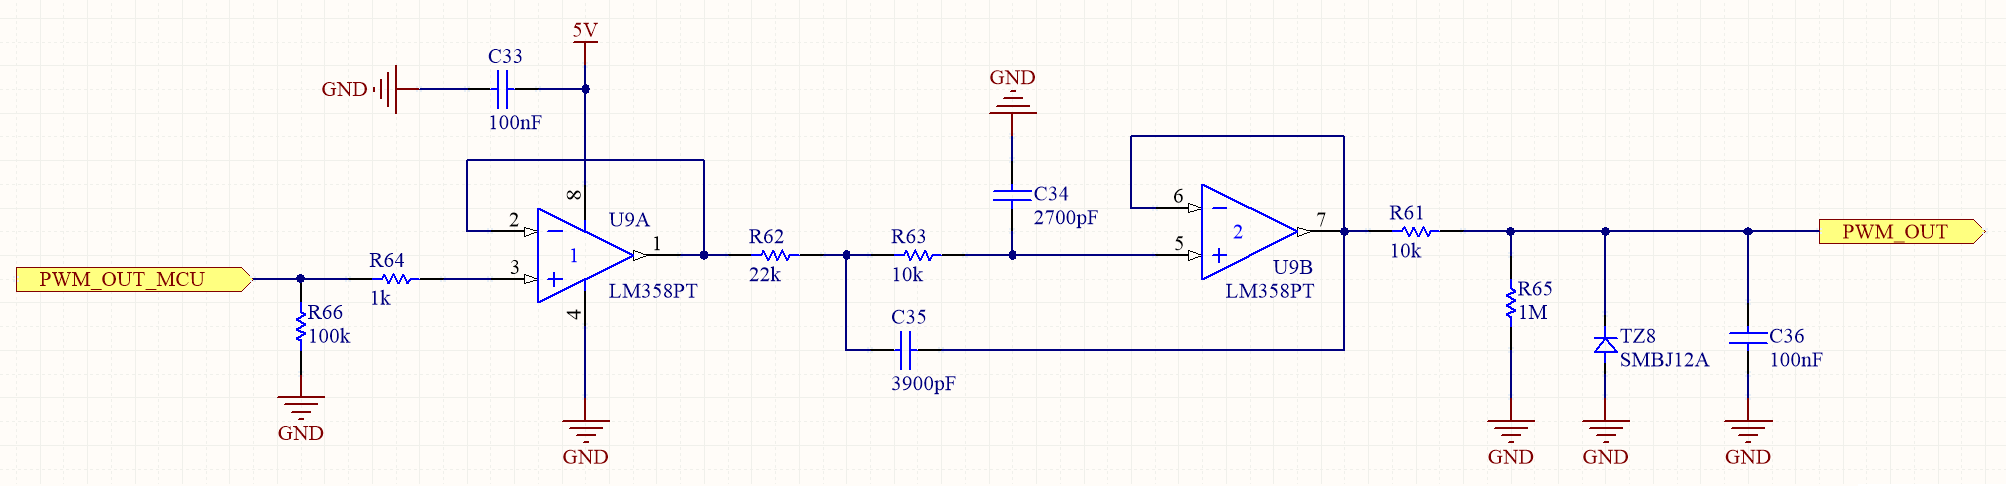
\includegraphics[scale=0.8]{figuras/fig-pwmToSpeedReferenceCircuit}
			\caption{PWM to Speed Reference Circuit}
			\label{fig:pwmToSpeedReferenceCircuit}
		\end{figure}
